\documentclass[UTF8]{article}

\usepackage{ctex}
\usepackage{geometry}
\usepackage{amsmath}
\usepackage{amssymb}
\usepackage{enumerate}
\usepackage{listings}
\usepackage{color}
\usepackage{graphicx}
\usepackage{hyperref}
\usepackage{tcolorbox}
\usepackage[english]{babel}
\usepackage[numbers]{natbib}
\usepackage{multirow}

\geometry{a4paper,left=2.5cm,right=2.5cm,top=2cm,bottom=2cm}
\setlength{\parindent}{0pt}

\title{Final Assignment - Academic English Writing}
\author{Ming Yang, The School of Data Science\\ \small{24210980134}}
\date{}

\begin{document}
	
\maketitle

\newtheorem{definition}{Definition}
\newtheorem{example}{Example}
\newtheorem{theorem}{Theorem}

\setcounter{page}{2}

\begin{tcolorbox}
  \textbf{Comment: } In this assignment, I will introduce the research proposal about 
  \textit{Nearest Neighbor Search} and \textit{Approximate Nearest Neighbor Search}, 
  which is a hot topic about articial intelligence. It is the techniques about how robots
  search some information automatically.
  It is a very hot topic in this field, I hope you guys can learn something new from this proposal.

  \textbf{Word Count: } 2436 

  \textbf{Citation Style: } IEEE
\end{tcolorbox}

\section{Introduction}
\textit{Vector embeddings} are a way to convert words and sentences and other knowledge into numbers (called \textit{vectors}) that 
capture their meaning and relationships (e.g., $\heartsuit \overset{\text{embedding}}{\implies} [0.124, 1.564, ...]$).
By convert words into numbers, the robots can understand the meaning of words and sentences. 
If AI(s) want to search information, they need to search the vectors most similar to the query word (vector), 
which is called \textit{Nearest Neighbor Search} or \textit{Approximate Nearest Neighbor Search}. For example, 
if an AI robot want to find some materials about \textit{Covid-19}, it needs to convert the word \textit{Covid-19} into a vector, 
that is a list of numbers, and then search the vectors most similar to the vector of \textit{Covid-19} in the dataset.
The similarity between two vectors can be calculated by the distance of them as shown in the following definition.

\begin{definition}[Vector Distance]
  Vector distance is a measure of the similarity between two vectors, which can be 
  calculated by the following function:
  $$
  dist(x, y) = \sqrt{\sum_{i=1}^{n}(x_i - y_i)^2},
  $$
  where $x_i$ and $y_i$ are the $i$-th number of vectors $x$ and $y$.
\end{definition}

If the distance between two vectors is smaller, the similarity between them is higher \cite{wang2024distance}.
After that, the definition of \textit{Nearest Neighbor Search} and \textit{Approximate Nearest Neighbor Search} are shown
formally as follows.

\begin{definition}[Nearest Neighbor Search, NNS]
  The algorithm aims to find some vectors in dataset with the smallest distance to the given query.
\end{definition}

It is becoming increasingly popular in various application domains \cite{arora2018hd}, 
such as information retrieval \cite{zhu2019accelerating}, 
pattern recognition \cite{kosuge2019object}, and retrieval augmented generation (RAG) \cite{brown2020language}. 
However, It is costly to find the exact nearest neighbors in practice, thus recent studies have focused on 

\begin{definition}[Approximate Nearest Neighbor Search, ANNS]
  It aims to find vectors with the smallest distance to the query 
  with efficiency while mildly relaxing accuracy constraints.
\end{definition}

Existing ANNS methods can be divided into four categories, including tree-based approaches \cite{arora2018hd}, 
hashing-based approaches \cite{huang2015query}, quantization-based approaches \cite{dobson2023scaling}, and graph-based approaches \cite{fu2017fast}. 
Among them, graph-based approaches stand out with the high answer quality and low latency. 
In the next parts, I will introduce four types of graph-based approaches, their search algorithms and design my method 
for the graph-based approach, which can improve the performance of the most mainstream graph-based approach.

\section{Literature review}
In this section, I will introduce four types of graph-based approaches and their search algorithms.
Before introducing the graph-based approaches, I will first introduce what is a graph and 
the \textit{Six Degrees of Separation} theorem. 

\begin{definition}[Graph]
  A graph $G = (V, E)$ is a pair of sets $V$ and $E$ such that each element of $E$ is a 2-element subset of $V$.
  The elements of $V$ are called nodes, and the elements of $E$ are called edges.
\end{definition}

\begin{example}[7-Node Graph]
  In the Figure~\ref{fig:pg}, there is a graph
  with 7 nodes (circles) and 7 edges (lines).
\end{example}

\begin{figure}[ht]
	\centering
	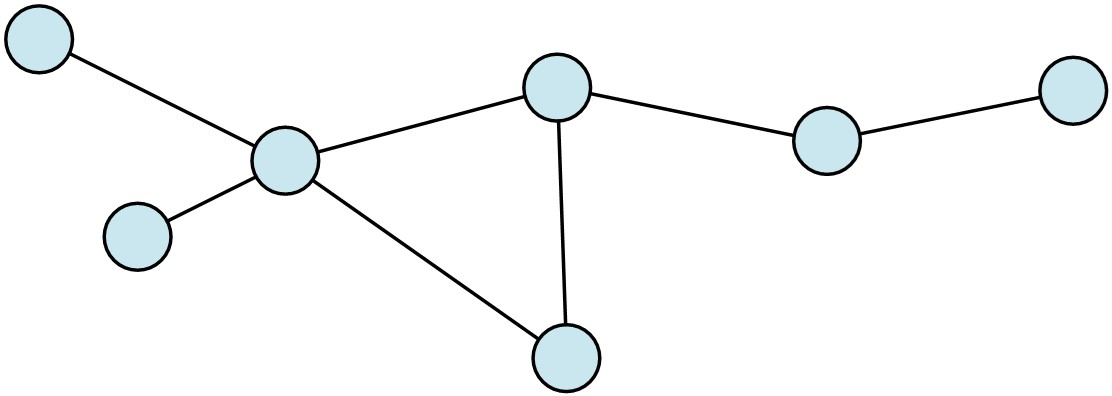
\includegraphics[width=.4\linewidth]{pg.jpg}
	\caption{The overview of the proximity graph.}
  \label{fig:pg}
\end{figure}

\begin{theorem}[Six Degrees of Separation] \label{thm::6d}
  There will be no more than six people between you and any stranger. In other words, 
  you can get to know any stranger through at most six people.
\end{theorem}

The \textit{Six Degrees of Separation} theorem is a well-known concept in social networks. 
It shows the power of graph-based approaches in connecting vectors.
By using graph-based approaches AI robots can find the query vector with high accuracy and low latency.

\subsection{Ideas of other graph-based approaches}

A \textit{Proximity Graph (shorten as PG)} is a graph where each vector is represented by a node in the graph, 
and each node is connected to its nearby neighbors 
(vectors are considered to be neighbors of each other if there exist an edge between them in the graph).
Current proximity graphs can be classified into four categories \cite{wang2021comprehensive}. 
\begin{description}
  \item[(1)] \textbf{Delaunay Graph (DG).} It ensures that for any edge, no other vectors will be situated within
  the hypersphere defined by an edge connecting two vectors, where the hypersphere is centered at the
  midpoint of the edge and the length of the edge is the diameter \cite{peng2023efficient}.
  \item[(2)] \textbf{Relative Neighborhood Graph (RNG).} It guarantees that for any edge between two vectors, no
  other vectors will reside within the lune constructed by the two \cite{flickner1995query}. 
  RNG imposes stricter restrictions on its edges, thus decreasing the average numbers of neighbors.
  \item[(3)] \textbf{K-Nearest Neighbor Graph (KNNG).} In KNNG, neighbors of each vector are its $k$
  nearest neighbors in the dataset \cite{dong2011efficient}.
  \item[(4)] \textbf{Minimum Spanning Tree (MST) Graph.} The MST utilizes distances between vectors as edge
  weights(value). Then, it performs hierarchical clustering on the dataset multiple times randomly, adding
  some edges \cite{zhou2013large}.
\end{description}

\begin{figure}[ht]
	\centering
	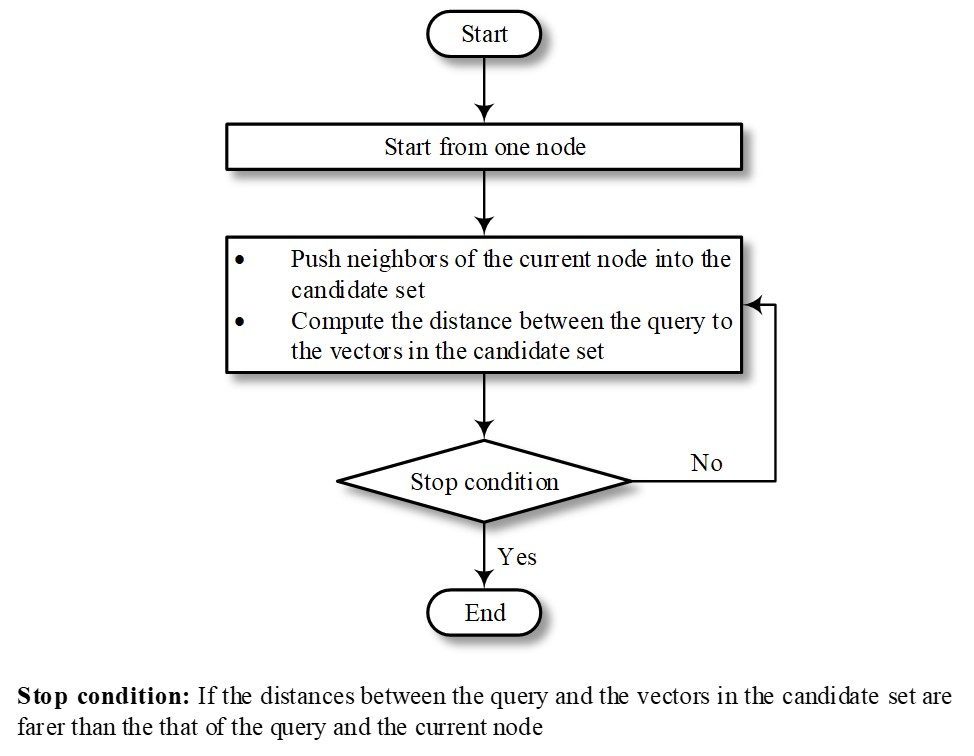
\includegraphics[width=.8\linewidth]{search_process.jpg}
	\caption{The search process of the graph-based ANNS.}
  \label{fig::search_process}
\end{figure}

The search algorithm is the core of the graph-based ANNS, 
which is used to find the query vector's neighbors in the graph.
The process is shown in Figure~\ref{fig::search_process}.
It is observed that the distance computation
dominates the overall time cost \cite{wang2021comprehensive, zhu2019accelerating}.
So the efficiency of the graph-based ANNS is highly dependent on the efficiency of the distance computations.
Due to the graph-based approaches and the Theorem~\ref{thm::6d}, graph-based methods can solve this well, 
because it can reduce the distance computations well by using the Six Degree Separation Theorem to find the query vector quickly.
That is the reason why with the development of AI, more and more efficient ANNS search algorithms are proposed,
and why the graph-based ANNS is still a hot topic.

\subsection{Inspiration from the literatures}
\textbf{\color{blue} These works give me some inspiration for my method, 
may be you can also find some: } Most well-known graph-based ANNS algorithms, e.g., HNSW \cite{malkov2018efficient}, 
do not exactly fit into one of the four categories. Instead, they usually evolve from one
or more of these proximity graphs \cite{dobson2023scaling}. And they are usually have a common feature, that is, 
to construct a graph with both long edges and short edges. In my opinion, this is a intuition for my method.
The long edges are often used in the early stage of the search process, 
because they can help to find the query vector's neighbors (nearby zone) quickly.
The short edges are often used in the late stage of the search process, 
because they can help to search the query vector's neighbors (nearby zone) accurately. 
On the other hand, if the graph search process can be divided to multiple stages, e.g., early stage and late stage,
then the algorithm can be optimized, instead of doing a parameters-fixed search for the whole process.

\section{Methods}

In the part, I will introduce my method, which is also a graph-based approach.
My method targets to improve the graph-based ANNS by using the partitioning strategy to reduce the number of distance computations.
Here are some details about my method and their reasons \cite{aumuller_ann-benchmarks_2020}. 
In Computer Science, a list of procedures is called an algorithm, which is a step-by-step procedure for solving a problem.
I then introduce the two key algorithms of my method, i.e., partitioning algorithm and search algorithm.

\subsection{Partitioning algorithm}
It is clear that I want to design an graph-based approach that can search as fast as possible and as accrate as possible \cite{gao2024rabitq}.
That means when the search process is far from the query, it needs to use a larger step to approach the query (for the speed), 
while when it is close to the query, it needs to use a smaller step to approach the query (for the accuracy).

The basic idea is randomly partitioning the
dataset $\mathcal{D}$ into multiple groups that share some common vectors, called \textit{routing vectors}. 
Then a sparser and smaller graph is built for each group of vectors. Since these each small subgraph are sparser than
that built for the whole dataset, allowing larger steps to approach the query quickly. 
Moreover, the routing vectors across multiple group enable efficient fine-grained search.

\vspace{-3mm}
\begin{example}[Partitioning strategy]
  In the Figure~\ref{fig::method}, the algorithm randomly divides the dataset $\mathcal{D}$ into two groups.
  Then it builds graphs for two groups, that are
  $\mathcal{G}_1$(left) and $\mathcal{G}_2$(right).
  The routing vectors are red ones, which are shared by two groups. The green ones are the vectors from 
  $\mathcal{G}_1$ and the blue ones are the vectors from $\mathcal{G}_2$.
  The query vector is noted as $\otimes$.
\end{example}

\begin{figure}[ht]
	\centering
	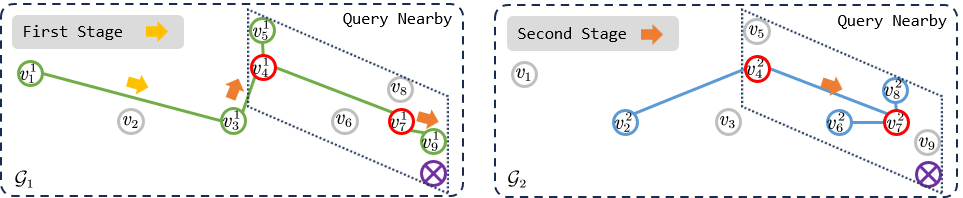
\includegraphics[width=.9\linewidth]{method.png}
	\caption{A example of my method.}
  \label{fig::method}
\end{figure}

\vspace{-3mm}
\subsection{Search algorithm}
The search process of my method is divided into two stages, i.e., fast approaching and precise search.
Specifically, the first stage aims to quickly approach the query vector by using only one proximity
graph, while the second stage will carefully search around by considering all groups for the
final closest vectors. Traditional beam search on a single proximity graph maintains a fixed-size
candidate set. In contrast, my method uses different sizes $ef_1$ and $ef_2$ for the two stages respectively,
where $ef_1 < ef_2$.

\subsubsection{The First Stage: exploring single partition for fast approaching}
In the first stage, the algorithm quickly approaches the query nearby with a shorter search length and
fewer neighbor expansions. It conducts a greedy beam search discussed in
the Figure~\ref{fig::method}. The yellow arrows indicates the first stage, while the orange arrows indicates the second stage.
The algorithm first starts the search from the $\mathcal{G}_1$, and after the first stage, the algorithm zones in the nearby region of 
the query vector, which is shown as the dot parallelogram in Figure~\ref{fig::method}. 
Then the algorithm continues the search from $\mathcal{G}_2$.
The second stage is a fancy technique that allows the search process to dynamically traverse different groups.

\subsubsection{The Second Stage: cross-partition expansion for precise search}
After the greedy search in the first stage, the candidate set contains the closest vector delivered in the
first stage from the first partition w.r.t. the query vector. It continues the greedy beam search with a size 
$ef_2$ for the candidate set. In the
second stage, the significant difference from the first stage lies in that: if the expanded
neighbor $u$ is a routing vector, all its instances in all partitions will be pushed into the candidate set. 
This approach allows the search process to dynamically traverse different proximity graphs, maximizing the search
space to include as many potential closest vectors as possible.
The search across multiple graphs in the second stage appears as though it is conducted
within a single proximity graph. In practice, with appropriate partitioning,
CSPG outperforms traditional PG algorithms.

\subsection{Experiment}
As summarized in Table~\ref{tab::dataset}, four benchmark datasets (SIFT1M, GIST1M, DEEP1M, SIFT10M) are used in the experiments, 
which are the most commonly used public datasets \cite{wang2021comprehensive}.

\vspace{-5mm}


% --- START OF FILE: dataset ---
\begin{table}[ht] 
  % \vspace{-4mm}
  \caption{Experimental Datasets} \label{tab::dataset}
  \centering
  \small
  \renewcommand{\arraystretch}{1.5}
  \setlength{\tabcolsep}{6mm}
  \begin{tabular}{crrrr}
  \hline
  \multicolumn{1}{r}{\textbf{Dataset}} & \textbf{Dimension} & \textbf{Data type} & \textbf{\# Base} & \textbf{\# Query} \\ \hline
  SIFT1M                        & 128                & float             & 1,000,000       & 10,000           \\ 
  GIST1M                        & 960                & float             & 1,000,000       & 1,000            \\ 
  DEEP1M                        & 96                 & float             & 1,000,000       & 10,000           \\ 
  SIFT10M                       & 128                & uint8             & 10,000,000      & 10,000           \\ \hline
  \end{tabular}
  % \vspace{-3mm}
\end{table}

% --- END OF FILE: dataset ---



And four types of graph-based ANNS algorithms are used in our experiments, 
including \textit{HNSW}, \textit{HCNNG}, \textit{Vamana} and \textit{NSG}.
My method in the following part, namely Crossing Sparse Proximity Graph (CSPG), is built upon each graph-based ANNS algorithm.

Figure~\ref{fig::perf} presents the QPS-recall curve of the my method built upon each graph-based ANNS
algorithm, comparing it with the corresponding traditional proximity graph implementation. 
There are two axes, i.e., QPS and Recall@10. 
QPS is the number of queries per second, 
which is the reciprocal of the average query time (shows the speed of the retrieval results) \cite{aumuller_ann-benchmarks_2020}. 
Recall@10 is the ratio of the number of retrieved vectors
to the number of ground truth vectors (shows the accuracy of the retrieval results) \cite{zhu2019accelerating}.
\textbf{If an algorithm achieve a higher QPS and a higher Recall@10, it means that the algorithm is faster and more accurate} 
\cite{kosuge2019object}.

\begin{figure}[ht]
	\centering
	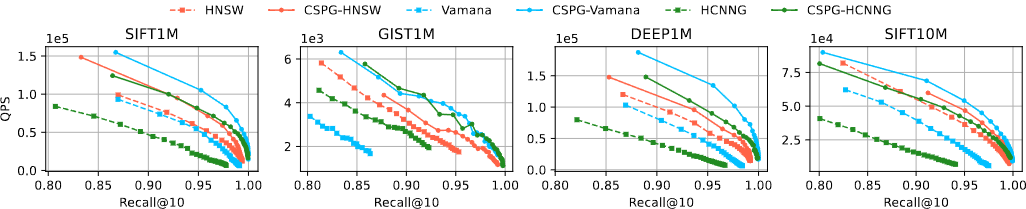
\includegraphics[width=\linewidth]{perf.png}
	\caption{QPS-Recall curve on the given dataset.}
  \label{fig::perf}
\end{figure}

For all datasets and graph-based algorithms, my method consistently improves the overall query performance.
Specifically, my method helps the \textit{Vamana} and \textit{HCNNG} indices to achieve at least 1.5x speedup on all the datasets.
It is clear that my method have a higher QPS and a higher Recall@10 than the traditional proximity graph implementation.

To show the Pareto frontiers (which is the optimal trade-off between QPS and Recall@10) of my method, 
I conduct a grid search experiment
to identify the most effective hyperparameter combinations for each baseline on SIFT1M dataset. 
Next, a more comprehensive
evaluation is conducted using the ANN-Benchmarks \cite{aumuller_ann-benchmarks_2020}, which is a widely used bench-
marking environment. For each algorithm, I choose the optimal param-
eters from the grid search experiment
with the highest QPS when $Recall@10 = 0.9 \pm 5e^{-3}$ on SIFT1M dataset. As
shown in Figure~\ref{fig::ann-benchmark}, enhanced with the
proposed CSPG framework, representative algorithms such as HCNNG, HNSW,
Vamana and NSG can achieve better performance on SIFT1M dataset

\begin{figure}[ht]
	\centering
	\includegraphics[width=.6\linewidth]{ann-benchmark.pdf}
	\caption{QPS v.s. Recall@10 curve on SIFT1M in ANN-Benchmarks.}
  \label{fig::ann-benchmark}
\end{figure}

\vspace{-5mm}
\section{Conclusion}
I propose a novel schema for approximate nearest neighbor search (ANNS), namely CSPG. 
By randomly partitioning the dataset, my method creates smaller, sparser proximity graphs for each partition and some routing vectors. 
I design an efficient two-stage search approach, combining fast proximity search and cross-partition precise expansion. 
In this way, my method can approach the query quickly by using a certain sparser and smaller graph, 
then it collects results precisely by crossing different partitions when it encounters a route vector.
The experimental results show that my method can achieve a higher QPS and a higher Recall@10 than the traditional proximity graph implementation.

\bibliographystyle{IEEEtranN}
\bibliography{ref}
\appendix
	
\end{document}